\documentclass[12pt]{article}
\usepackage[paper=a4paper,margin=2.5cm]{geometry}
\usepackage{titling}
\usepackage[colorlinks=true]{hyperref}
\usepackage{enumerate}
\usepackage{amsmath}
\usepackage{enumitem}
\usepackage{graphicx}
\usepackage{subcaption}
\usepackage{pdflscape}
\usepackage{longtable}
\usepackage{fancyhdr}
\setlength{\parskip}{12pt}
\usepackage{setspace}
\setstretch{1.5}

\setlength{\droptitle}{-6em}

\title{Term Paper STV2022}
\author{Candidate Number: 17112}
\date{Fall 2022}



\begin{document}
\pagestyle{fancy}
	\lhead{Fall 2022}
	\chead{STV2022}
	\rhead{Candidate Number: 17112}
	\lfoot{ }
	\cfoot{\thepage}
	\rfoot{ }
	\setlength{\headheight}{15pt}
	

	\begin{titlepage}
		\begin{center}
			\vspace{1cm}
			
			\Huge
			\textbf{Speaking for their gender: Patterns of substantive representation of women's issues in the Norwegian Parliament}
			
			\Large
			Term Paper \\
			STV2022 - Store Tekstdata 
			
			\vspace{2cm}
			
\includegraphics[width=0.4\textwidth]{1245071}
			
			\Large
			Fall 2022 \\
			Candidate Number: 17112
			
			\vspace{2cm}
			Word count: 3942
			
		\end{center}
	\end{titlepage}
	
	\section{Introduction: Research Question and Hypotesis}
	
	Political representation is understood in broadly speaking two manners, one is the degree to which an assembly of political representatives resembles the people they are meant to act on behalf of, this is what is known as descriptive representation (Pitkin, 1967). The other form usually studied, which Pitkin herself promotes is that of substantive representation, constitutes the actions committed on behalf of their constituents. The actions themselves become what constitutes representation. According to Pitkin (1967) these are distinct understandings of representation, but as later pointed out, descriptive representation may be a necessary condition for substantive representation (Phillips, 1995).
	
	This connection has garnered much attention in recent years (Wangnerud, 2009; Blumenau, 2021), and this paper will attempt to shed further light on this issue, using newly collected data, as well as machine learning for textual analysis, which has been underutilised in this literature. The main goal of the paper is to utilise topic modelling to create a quantitative measure of women's issues that comes closer than general topics previously used. I will attempt to answer the following question:
	
	\begin{quotation}
		\textit{Do Women Representatives perform more substantive representation than men on behalf of women?}
	\end{quotation}
	
	In order to answer this question I will utilise data from the Norwegian parliament. The Norwegian case is useful due to its high levels of women's representation, as well as general history of gender equality. Previous research have also used data from the storting, along with similar model choices, to connect substantive representation to regional responsibilities (Finseraas et al, 2021).
	
	\subsection{Operationalization and Hypothesis}
	
	The first step is to clarify what is meant by women's issues, as the concept itself has been heavily debated (Celis et al, 2014). I take a broad approach to clarify them as issues that are primarily of exclusive relevance to women, but also on issues that have significant history of relevance for women, despite nominally being about men too. Exclusive relevance then means issues such as pre-natal healthcare and abortion rights, while history of relevance is connected to issues such as wage-gap. 
	
	My main expectation is rooted in previous observations (Blumenau, 2021), which is that women representatives will focus more of their speech acts on issues that affect women, will dedicate more attention to it, and will account for a larger proportion of the discourse around these issues, than their male counterparts. This theory is rooted in experiences from many scholars (Wangnerud, 2009), and is largely attributed to either party-strategic decisions, or individual choices of political interests of the representatives. Regardless, it is also seen as a normative question, whether or not women are needed in order to provide sufficient attention to these issues, and while this paper makes no claim as to what is an optimal amount of attention, it will hopefully provide clarity as to whether such a goal could be met by increasing the amount of women representatives. 
	
	The mechanisms behind this potential effect has also been widely discussed. Women, or members of other political minorities, have direct and first-hand knowledge of difficulties that they face, and are therefore more sympathetic to those causes (Phillips, 1995). But they are also in general, better at communicating these issues (Mansbridge, 1999).
	
	\section{Data: Collection and pre-processing}
	
	The data was collected using the stortings API, through the package stortingscrape, created by Søyland (2022). This package allows for seamless usage of the storting API through R. I only studied questions, due to the large amount available, but also because I believe it represents the genre of speech acts that give the most independence to the individual representative, and the least affected by party orders.
	
	\subsection{Data Collection}
	
	I decided to take advantage of as much of the data as I could possibly get my hands on, and as such I tested the limits of what was available to the Stortings API. It quickly became clear that only data going back to 1996 was available for scraping. I believe this is still sufficient for the task at hand, given that it covers a variety of government constellations, and several elections. Regardless of time limit the workflow with the API for the Storting is as follows: 
		
	\begin{enumerate}
		\item Collecting data on the sessions and their id numbers
		\item Collecting the meta information on all questions in the sessions
		\item Using this meta data to scrape the actual text of each question
		\item Separately, the relevant MP's for the sessions must be found
		\item When found, their relevant information is joined with the dataframe containing all the questions.
		\item At this point we have our structured Data.
	\end{enumerate}
	
	The attached R-script details how this was accomplished by utilising different functions from the Stortingscrape package, which yielded a dataframe of 52856 questions, containing texts of questions, justifications and answers, along with meta data for the representative and the question. 
	
	There is a discussion to be had in regards to separating the answer from the question, given that they are not formulated by the same individual. However, genre coherence gives reason to believe that these will be similar, and that including the answer in all questions would yield a similar genre to all questions. The questions are genre-coherent at two important levels, that of question structure itself, which is important given that the primacy lies with the question asker in all cases to decide what the topic itself is. The answer will by necessity belong to the same topic, and the data-generating process by which a topic is made, lies primarily with the asker. Secondly, the question all share the same arena, that of political life in Norway, more specifically the formal setting of the Storting. Lastly, having more texts is likely to help the eventual machine learning model to make better judgements.
	
	The process itself went by without much flaws, except for the data having missing identification variables on questions from 1996, leaving the id, and subsequently gender of the person asking those questions as missing. In addition, 2 636 questions had empty texts, and consequently disappeared in the final dataframe after processing the texts of these variables. A quick inspection of the time spread of these questions reveal no apparent connection, so I assume this can be attributed to random errors.
	
	\subsection{Pre-Processing}
	
	Given that my stated goal is to run topic modelling on the documents themselves, I need to first tokenize the text, then remove the relevant stopwords in order to trim unnecessary information, then stem the words to create equivalent classes, and then finally cast a dfm function that creates a data frame where each document is a row, and each term a column (Grimmer et al, 2022, p. 52-54). This dfm is the input of our future LDA model. 
	
	The first step, is to tokenize the text. I do this by creating unigrams, splitting each isolated word into a token (Grimmer et al, 2022, p. 52). This splits the text up into singular isolated words, but retains their origin. Unigrams are the most basic form of splitting a big text up, as it pays no attention to the relationship between words internally in the text given. I first combine the question, justification and answer text into one. This is then tokenized into unigrams, split into individual words that make up the texts.
	
	The next step is to remove the relevant stopwords. In this instance I choose to use a tf-idf model to select away the terms that most frequently appears across documents in the corpus (Grimmer et al, 2022, p. 75). This model is created through the bind\_tf\_idf function in R. This provides a ranked list of terms to use for selecting away recurring terms, here a subjective assessment is needed, to decide a suitable cut-off point. I find the verb "to secure" which I deem to be possibly relevant to future topic modelling, and decide to use that as a cutoff point, and items with lower tf-idf score than that are listed as "stopwords". I then remove all of those matching words from the complete tokenized list, which leaves me with about 11 200 000 tokens, instead of the 20 million I previously had. 
	
	Following this, I stem the words using the Quanteda package. This is unfortunately sub-optimal as stemming is a very crude and simplistic method of simplifying words, but it does have it's advantages, namely the low computational requirement, and the uncomplicated implementation. Finally the stems are used to create a document feature matrix, or dfm, which will be the input in a structural topic model.
	
	Below are illustrations of aspects of the text before and after the relevant pre-processing steps. First I demonstrate the differences in Zipf's law in figure 1. Zipf's law states that the logarithm of the frequency a term is used, is inversely correlated with the logarithm of its rank. This is illustrated in the plots in figure 1, which shows the straight line as perfect correlation.
	
	\begin{figure}[h]
		\begin{subfigure}[b]{0.3\linewidth}
			\includegraphics[scale=0.40]{Img/Zipf\_law\_1.PNG}
		\end{subfigure}\hspace{3cm}%
		~  
		\begin{subfigure}[b]{0.3\linewidth}
			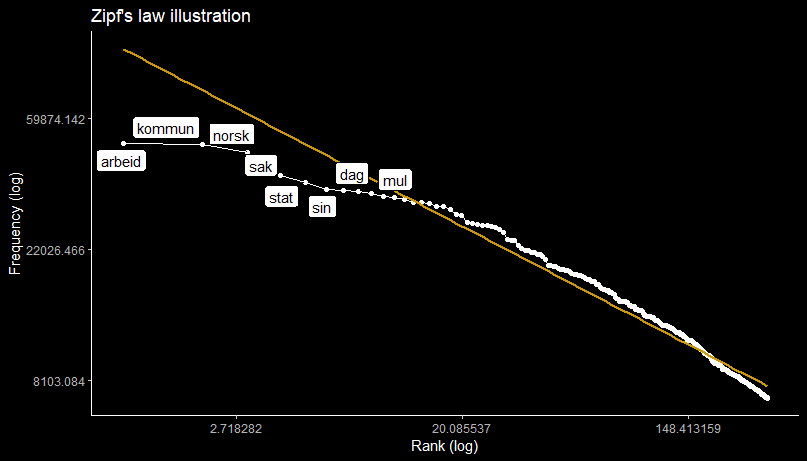
\includegraphics[scale=0.40]{Img/ziplaw2.PNG}
		\end{subfigure}
	\caption{\textit{Zipf's law, before stopword removal (left) and after (right)}}
	\end{figure}
	
	As demonstrated, the process did not yield perfect results, but it is a slight improvement, as it approaches the lines faster than the pre-processed data would. 
	
	Next is illustrated the reduction in length. The models clearly demonstrate a significant reduction in length for each genre of questions. Note that the plots are separated because the different types of questions vary greatly in length.
	
	\begin{figure}[ht]
		\centering
		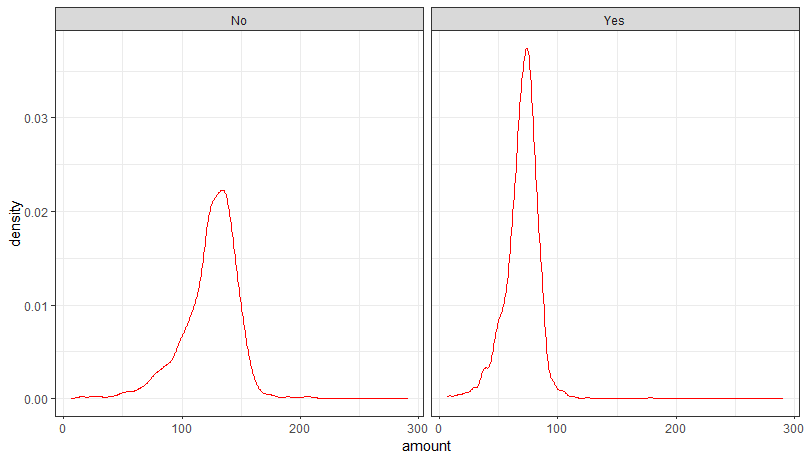
\includegraphics[scale=0.40]{Img/preposttreatedinterpell.PNG}
		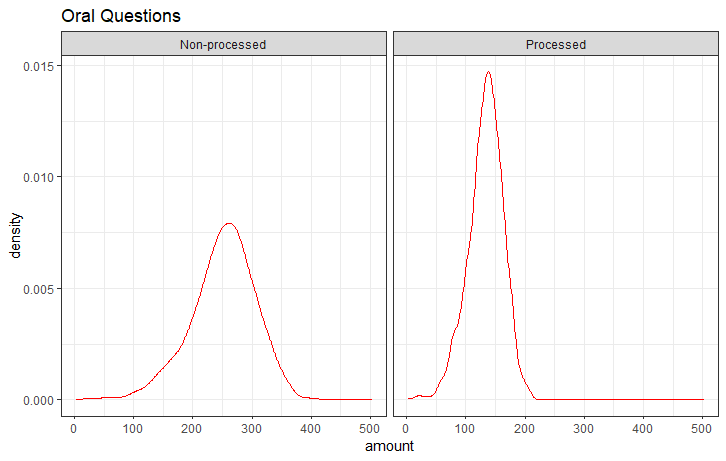
\includegraphics[scale=0.40]{Img/prepostmuntligsporsmal.PNG}
		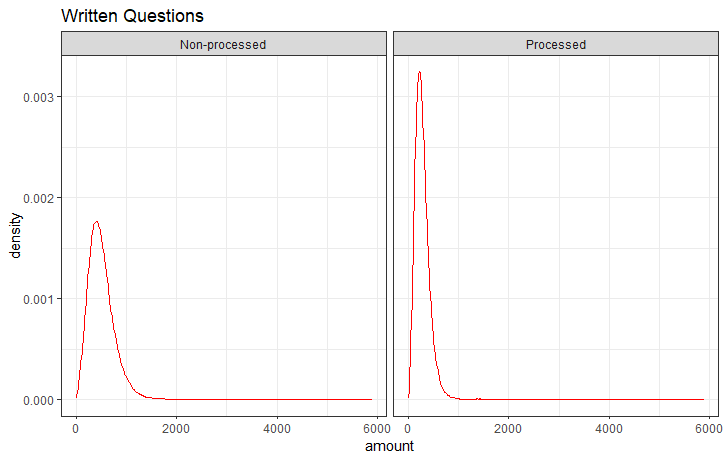
\includegraphics[scale=0.40]{Img/prepostskriftligsporsmal.PNG}
		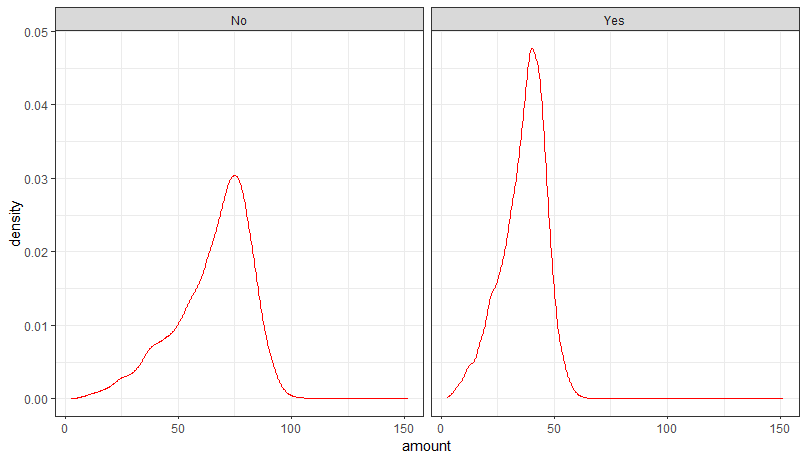
\includegraphics[scale=0.40]{Img/prepostsporretimesporsmal.PNG}
		\caption{\textit{Pre- and post-processed distribution of length of each document}}
	\end{figure}
	
	\subsection{Assessing the pre-processing}
	
	This process would eventually reveal several flaws later in the project, highlighting the need to inspect the results from any such process. Primarily, the eventual topic model singled out three New-Norwegian topics, all consisting of simple stopwords, that should have been removed. This is due to the tf-idf way of taking out stopwords, and it should have been backed up by the usage of snowballC's stopwords as well, but this mistake was not spotted until after the models were run, and that process itself took several days.
	
	Furthermore, the usage of stemming as opposed to lemmatization with more advanced processes revealed other issues. First there is the lack of contextual variety in some of the terms, meaning some tokens may have different meanings, despite being identical to others. The other main issue is that stemming applies a set of rules that sometimes removes the entire meaning of a word. The main example in this context is the word "fastlege" which is general practitioner. In our data this is stemmed to "fast" which shares identity with the word for permanent, or fixed. This may have severe impact on topics regarding health, and may impact issues of women's health. Another issue is that the adjective "possible" is stemmed to the same stem as the noun for "possibility", this is likely a problem in English as well.
	
	\section{Analytical strategy}
	
	To analyse this large corpus of questions, I chose to utilise a structural topic model, a type of unsupervised machine learning. This allows me to identify underlying topics in the texts, that are often recurring. The advantage of this strategy is its ability to draw out underlying associations, and see connections between different words. 
	
	The first challenge is then when the model has been specified and estimated, to retrieve the topics that I identify as belonging to the general topic of "women's issues". To do this I inspect all the resulting topics from my optimal model, and ascertain whether they cover issues regarding women's health, discrimination, women's reproductive health, and similar. It is difficult to know beforehand what could potentially be relevant, and it is largely something that has to be found after the model is estimated.
	
	After finding these topics, the next task is to extract the gamma values from the structural topic model's estimation. These gamma values represent the topic-proportion of each document, meaning how much of the document that the model estimated belongs to each topic. These values form the bulk of my strategy, as they can be interpreted as representing the probability that a document belongs to a topic. 
	
	I chose three approaches to interpret the results of the topic model. First I will illustrate the raw difference in these gamma values for each topic, for women and men. Secondly, given that these values tend to be bunched up close to zero due to the high amount of topics included, I also extract the questions that have the highest probability of belonging to the topic, meaning the questions that we are most certain are about women's issues. Demonstrating the distribution of gender on this indicates how prevalent women are in these discussions, but they may not capture whether or not women representatives use some of the language that is connected to the topics. While main topics reveal a focus on general women's issues, lower charges may reflect application of the language of those issues in other related issues. 
	
	The last approach then is to run a regression model on the relevant topics. Given the nature of the dependent variable, a number between 0 and 1 reflecting a general topic probability, ordinary OLS is insufficient (Ward \& Ahlquist, 2018, p. 50), as it may predict values of more than or less than 100\% or 0\% respectively. For this reason, I utilise the general logit framework, but because the data is technically not a Bernoulli trial format, I manually transform the probabilities into logit scale, and then run a normal regression on the results. This is done through the formula reported below, where the accumulated probabilities $P$ are transformed into logit values $Z$, which is the dependent variable in my regressions. 
	
	\begin{equation}
		logit(P) = log \frac{p}{1-p} = Z
	\end{equation}
	
	I also account for potential biases in party level data by including party as a control variable, and interacting it with gender. This will also yield a general outline of the role that women within parties play when it comes to performing representation of women's issues. 
	
	The dependent variable used for this process will be the combined document probabilities of the topics that are deemed to be relating to women's issues. The value of these combined will reflect what "portion" of the question is related to women's issues. The dependent variables is still between 0 and 1, because the cumulative topic-probabilities will always be 1, since they represent proportions of the texts. This makes them highly suited to logistical regressions. 
	
	\subsection{Potential Weaknesses of the chosen strategy}
	
	The advantage of the strategy chosen is that we could potentially receive a rather clear cut answer to the question, by simply looking at the resulting estimated effect that the model spits out. However, even if it is significant caution should still be excercised, and some issues should be addressed. The first issue has to do with the old adage "All models are wrong, but some are useful", a quote sometimes directly attributed to George Box. This quote is even more appropriate when discussing quantitative text analysis. While topic models might functionally be understood as uncovering "topics", what they actually uncover are concurrent incidents of word pairs, or word groups. Therefore, any analysis should always be critically interpreted, and researchers should be aware of what the model actually says, in addition to the underlying factors it hopefully reflects.
	
	The second issue has to do with the reliability of creating a unified understanding of "women's issues". By its very nature, it is difficult to sort that without having first viewed the data, but when viewed, the topics that are deigned to belong to that overarching meta-topic should be presented and properly argued to belong to the grouping. 
	
	Finally, a potential weakness of this strategy is the potential of failing to uncover the topics themselves. The model would require some fine tunings in order to accurately find all the relevant topics, and there is no guarantee that any amount of tuning will inevitably lead to an accurate isolation of my topics of interest. 
	
	\section{Empirical Results}
	
	A preliminary search was used, utilising the searc\_K function in the stm package. This yielded the results as demonstrated in the plot figure 2.
	
	\begin{figure}
		\centering
		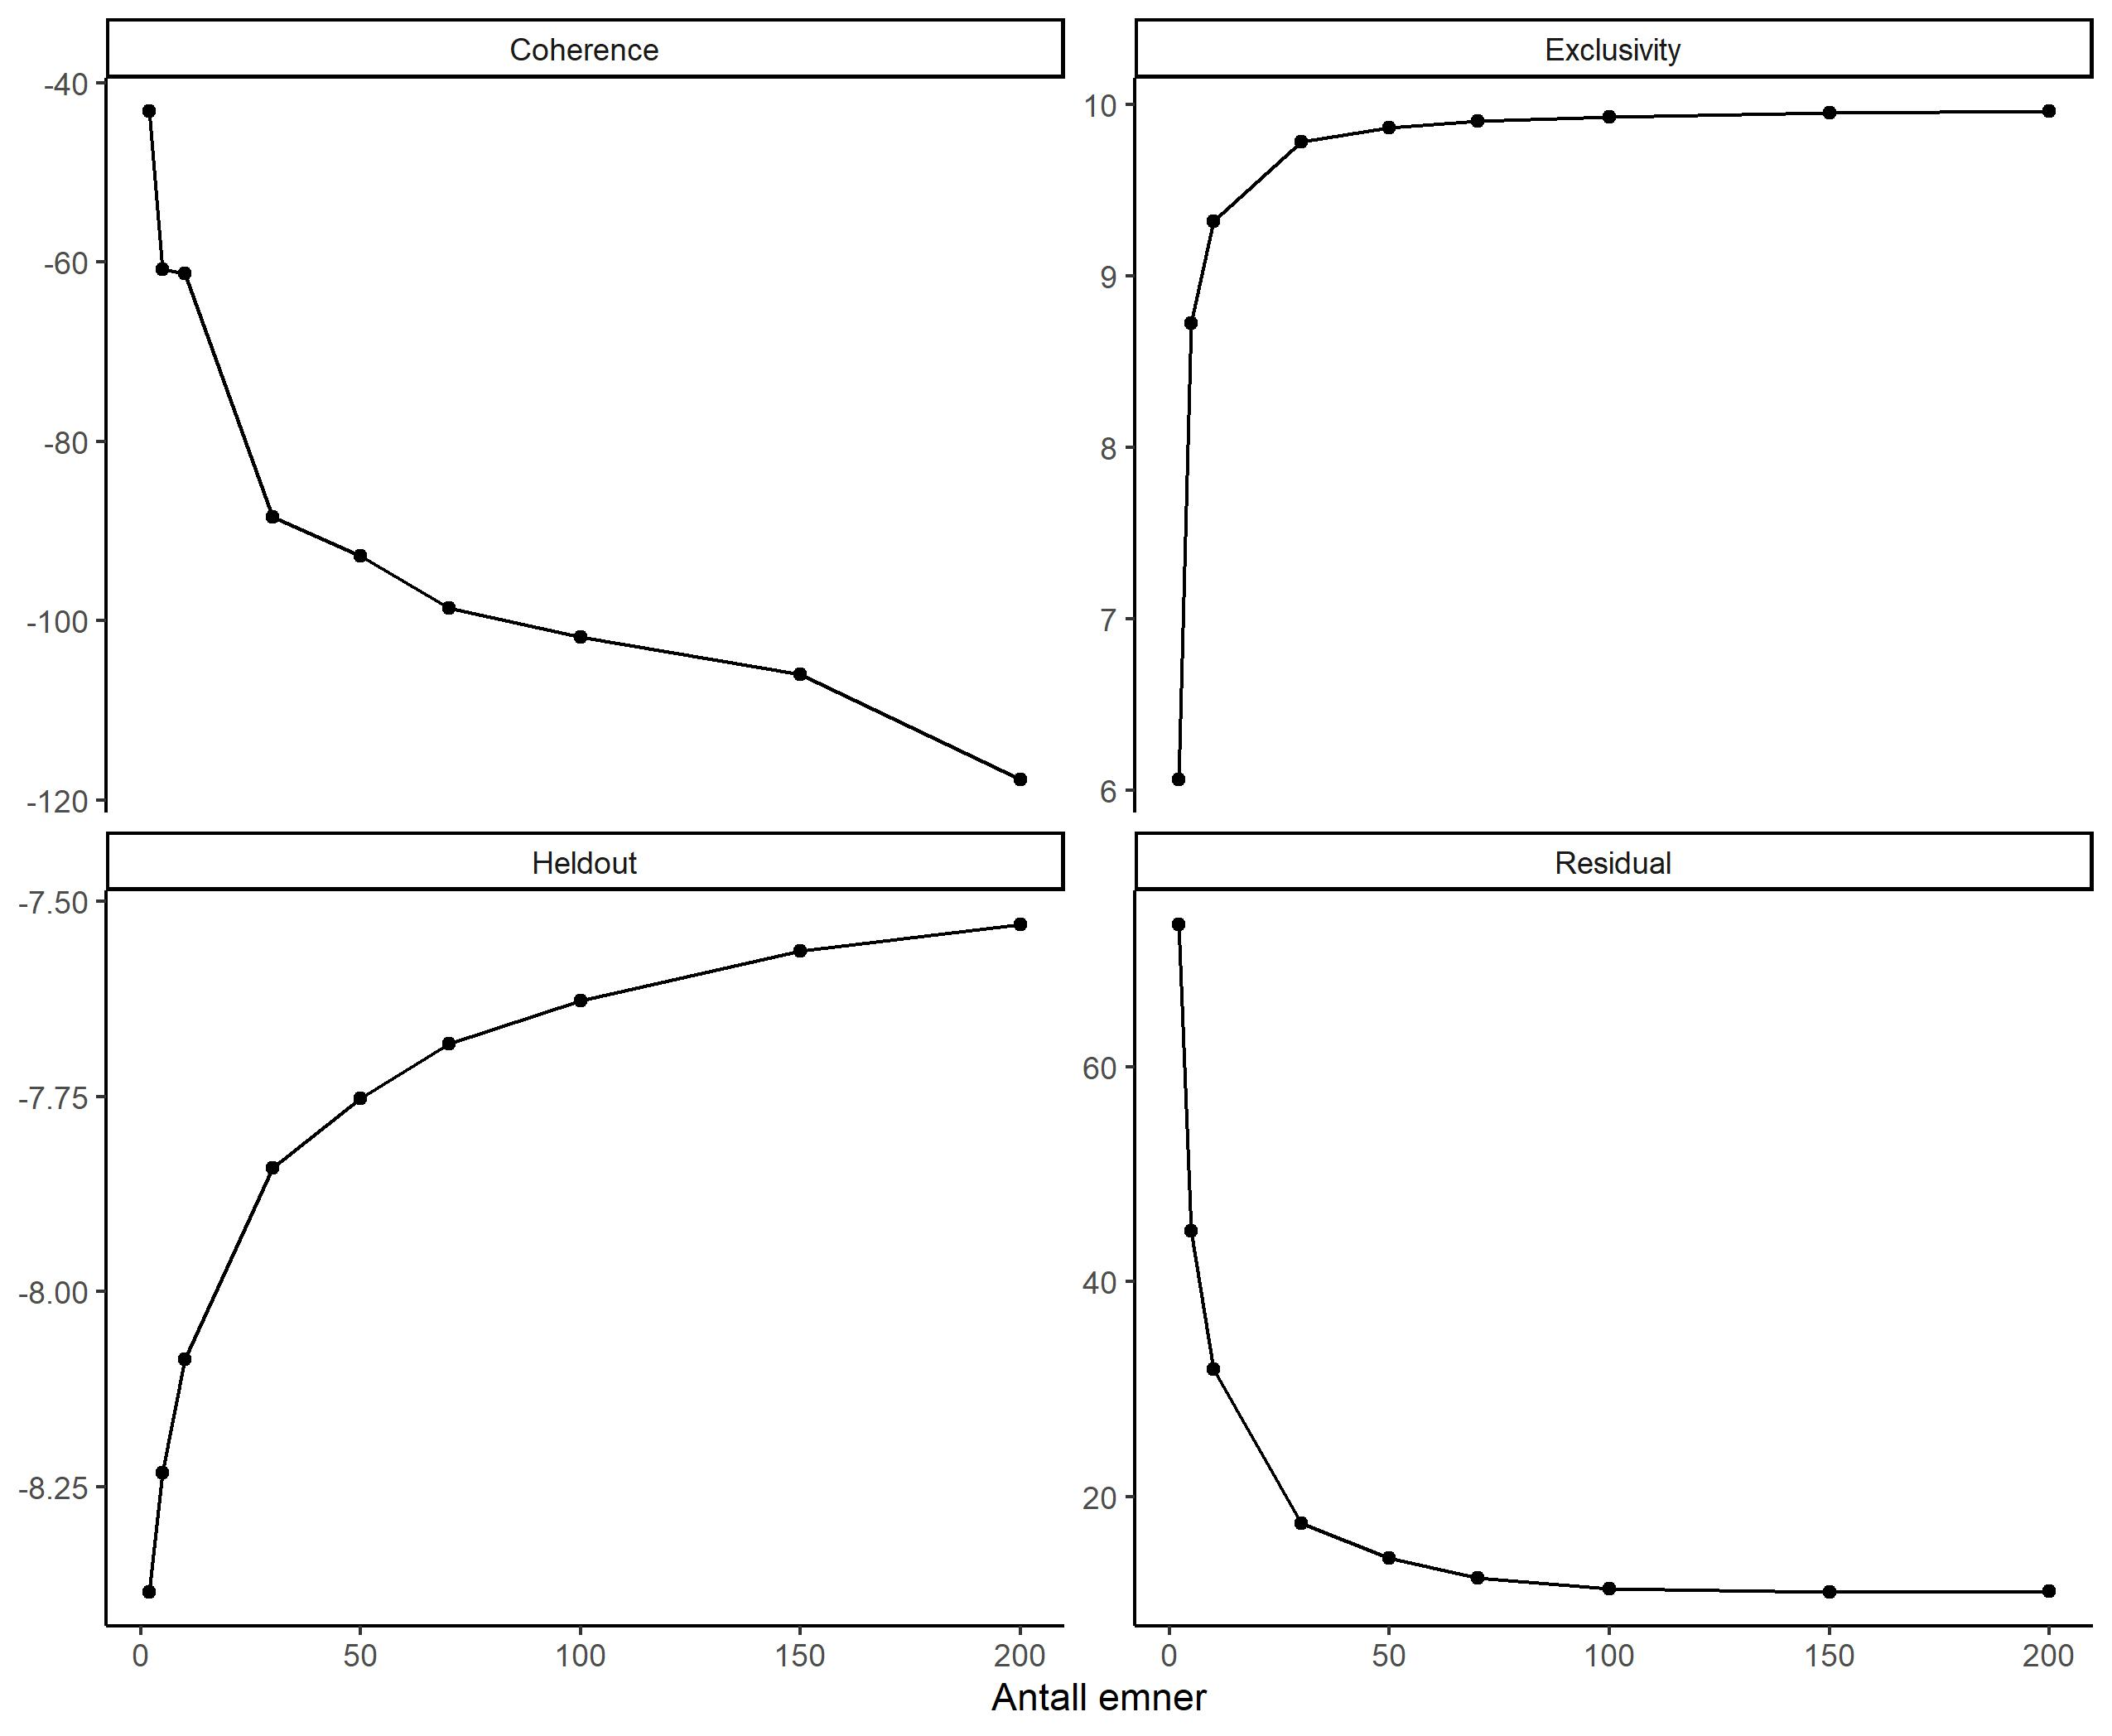
\includegraphics[scale=0.60]{ksearch.jpg}
		\caption{\textit{Results from topic searches}}
	\end{figure}
	
	While the model seem to indicate an optimal input at around 100 topics, while estimating, that model failed to report a substantial amount of topics related to women's issues, while the 200 topics model did. For that reason I chose a higher amount of topics to catch all the topics I was interested in. Therefore the model was estimated with 210 topics. This approach reflects an essential tenet of utilising machine learning, which is that subjective judgements are sometimes necessary for the model to be useful, and while all models are wrong, it is our job to ensure that our model is at the very least useful. This choice then yielded five topics relevant to women's issues.
	
	These are topics 119, 135, 138, 158 and 164 in the model output itself, which I label as being Pregnancy healthcare, gender equality, genital mutilation, forced marriages, and abortion and parental rights. I will refer to Main Topics as meaning pregnancy healthcare, gender equality and abortion, while the remaining two are more peripheral, and not necessarily "women's issues" primarily, especially since genital mutilation is probably more closely linked to immigration. These topics are represented in the word clouds in figure 3, where the size of the word represents its influence on the topic-proportion as a whole.
	
	\begin{figure}[h]
		\caption{\textit{Topics relevant to "women's issues"}}
		\begin{subfigure}{0.3\linewidth}
			
\includegraphics[scale=0.40]{topic119wordcloud.png}
		\end{subfigure}
		\begin{subfigure}{0.3\linewidth}
			
\includegraphics[scale=0.40]{topic135wordcloud.png}
		\end{subfigure}
		\begin{subfigure}{0.3\linewidth}
			
\includegraphics[scale=0.40]{topic138wordcloud.png}
		\end{subfigure}
	\end{figure}
	
	\begin{figure}[h]
		\centering
		\begin{subfigure}{0.45\linewidth}
			
\includegraphics[scale=0.40]{topic158wordcloud.png}
		\end{subfigure}
		\begin{subfigure}{0.45\linewidth}
			
\includegraphics[scale=0.40]{topic164wordcloud.png}
		\end{subfigure}
	\end{figure}
	
	\subsection{Raw difference in means}
	
	Below is a table that illustrates the differences in the mean value of each group. As is clearly evident, the group for women has between two to three times higher average score on the document proportion of their questions. This indicates that on average, women utilise more of the words that are associated with these topics, the words that are presented in the wordclouds above. 
	
	% latex table generated in R 4.2.1 by xtable 1.8-4 package
	% Thu Nov 10 19:42:20 2022
	\begin{table}[ht]
		\centering
		\caption{\textit{Raw differences in averages}}
		\begin{tabular}{rlrrrrr}
			\hline
			& Gender & top119 & top135 & top138 & top158 & top164 \\ 
			\hline
			Group.11 & Women & 0.00483 & 0.00448 & 0.00180 & 0.00246 & 0.00376 \\ 
			Group.12 & Men & 0.00141 & 0.00141 & 0.00098 & 0.00134 & 0.00156 \\ 
			\hline
		\end{tabular}
	\end{table}
	
	But this does not account for potential instabilities in parties, and whether or not this is just evidence that parties that have more women, also have a more feminist ideology. I will investigate these claims further in the next sections.
	
	\subsection{Time spread over the highest charging questions}
	
	The previous section suffers from the fact that questions in general charge very little on the topics that I am interested in. For that reason I choose to illustrate the general trend through picking out the highest charging documents for each of my main topics. These plots are illustrated below. Note the red represents women's portion of the questions, and blue is men.
	
	\begin{figure}[h!]
		\centering
		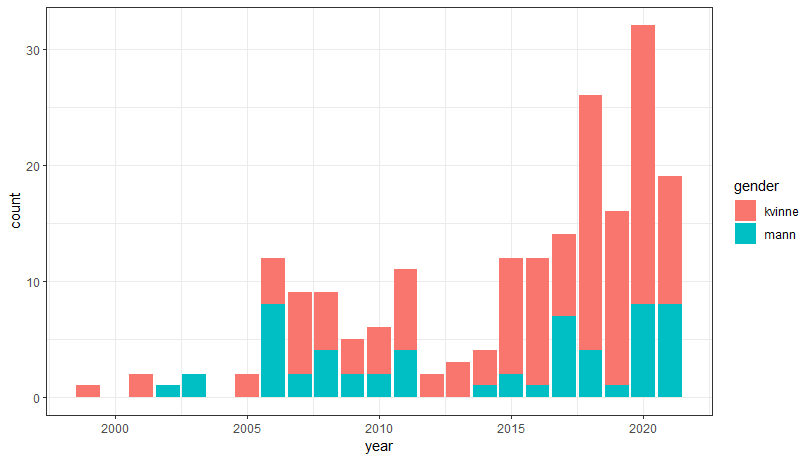
\includegraphics[scale=0.60]{Img/119dist.png}
		\caption{\textit{Gender distribution on highest charging pregnancy healthcare questions}}
	\end{figure}
	\begin{figure}[h!]
		\centering
		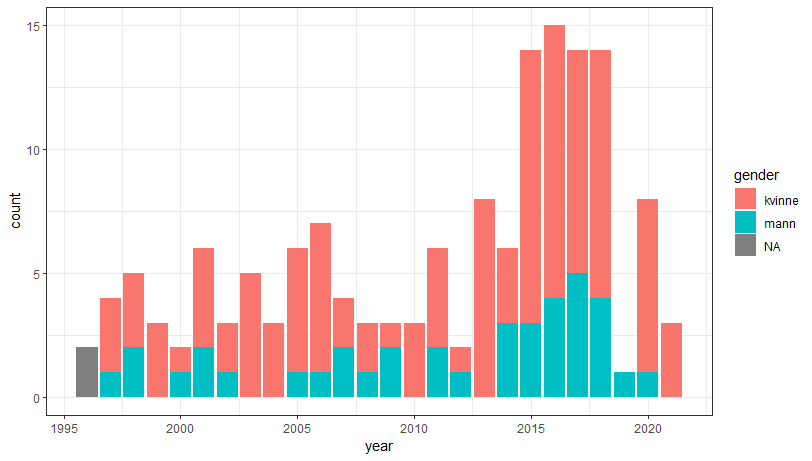
\includegraphics[scale=0.60]{Img/135dist.png}
		\caption{\textit{Gender distribution on highest charging gender equality questions}}
	\end{figure}
	\begin{figure}[h!]
		\centering
		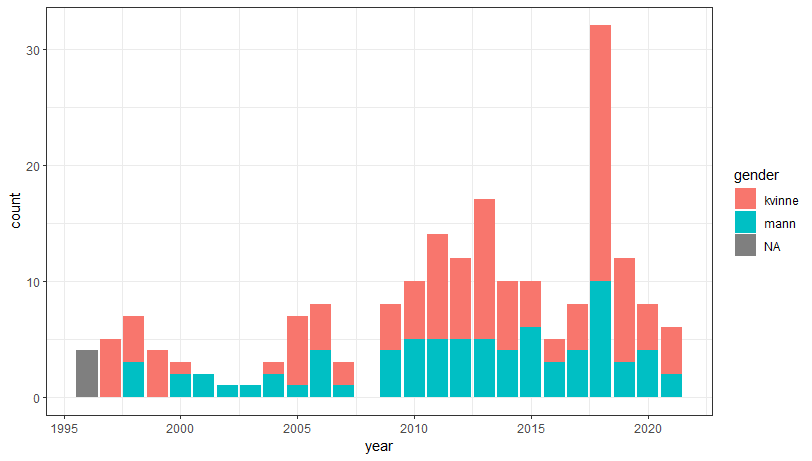
\includegraphics[scale=0.60]{Img/164dist.png}
		\caption{\textit{Gender distribution on highest charging abortion related questions}}
	\end{figure}
	
	
	The main thing to take note of is that women constitute a majority of the questions asked of all the main topics presented here. There seems to be a mild time trend, increasing, the other minor observation, is the massive increase in questions regarding abortions in the 2018-2019 session. This is most likely due to the ongoing internal strife in the Christian Democratic Party, where the Prime minister Solberg had at the time promised them to potentially revise the abortion laws if they entered into a coalition with her parties (Johnsen \& Skjetne, 2018). 
	
	\subsection{Regression on Topic probabilities}
	
	The final analysis is applying a logit regression, this will demonstrate whether gender is influential for the probability that a topic is related to women's issues, even controlling for party. I use two dependent variables, one combining the main topics, and one combining all relevant topics. I run three regressions on both of these, to see differences in controlling for party and party interaction with gender. I report the result of all these regressions in table 2 below, models 1 and 4 are with gender only, 2 and 5 are controlling for party, and 3 and 6 are with an interaction with gender and parties. The full regression table is reported in the appendix. 
	
	Evident from the regression is that gender plays a significant role, regardless of the model or the dependent variable. This demonstrates that women utilise significantly more language related to women's issues in questions that they pose to the relevant minister. Inspecting the full regression table also reveals that many conservative parties have significant and positive interactions with gender, meaning that the women of these parties are more active than their male party fellows. Additionally, only one party appears to have a gender party interaction that discounts the general party trend, which is the Red party. This means that almost regardless of party, women speak significantly more than men on these issues, and therefore perform more representation of women. 
	
	% Table created by stargazer v.5.2.3 by Marek Hlavac, Social Policy Institute. E-mail: marek.hlavac at gmail.com
	% Date and time: Wed, Nov 30, 2022 - 13:21:19
	\begin{table}[!htbp] \centering 
		\caption{\textit{Results of Logit Regression Models}} 
		\label{} 
		\begin{tabular}{@{\extracolsep{5pt}}lcccccc} 
			\\[-1.8ex]\hline 
			\hline \\[-1.8ex] 
			& \multicolumn{6}{c}{\textit{Dependent variable:}} \\ 
			\cline{2-7} 
			\\[-1.8ex] & \multicolumn{3}{c}{Logit.WTop1} & \multicolumn{3}{c}{Logit.WTop2} \\ 
			\\[-1.8ex] & (1) & (2) & (3) & (4) & (5) & (6)\\ 
			\hline \\[-1.8ex] 
			Female & 0.583$^{***}$ & 0.571$^{***}$ & 0.411$^{***}$ & 0.553$^{***}$ & 0.558$^{***}$ & 0.373$^{***}$ \\ 
			& (0.015) & (0.017) & (0.033) & (0.016) & (0.017) & (0.033) \\ 
			& & & & & & \\ 
			Constant & $-$7.878$^{***}$ & $-$7.752$^{***}$ & $-$7.662$^{***}$ & $-$7.389$^{***}$ & $-$7.308$^{***}$ & $-$7.203$^{***}$ \\ 
			& (0.009) & (0.019) & (0.025) & (0.010) & (0.019) & (0.025) \\ 
			& & & & & & \\ 
			\hline \\[-1.8ex] 
			Observations & 50,220 & 50,220 & 50,220 & 50,162 & 50,162 & 50,162 \\ 
			R$^{2}$ & 0.027 & 0.046 & 0.052 & 0.024 & 0.044 & 0.049 \\ 
			Adjusted R$^{2}$ & 0.027 & 0.046 & 0.051 & 0.024 & 0.043 & 0.049 \\ 
			\hline 
			\hline \\[-1.8ex] 
			\textit{Note:}  & \multicolumn{6}{r}{$^{*}$p$<$0.1; $^{**}$p$<$0.05; $^{***}$p$<$0.01} \\ 
		\end{tabular} 
	\end{table} 
	
	\section{Discussion}
	
	The findings imply a significant relationship between the substantive representation of women's issues and the descriptive representation of women. However, these findings are not without potential criticisms. While the regression analysis unequivocally confirms that on average, women utilise more language that imply they are performing representation on behalf of women, this could have other causes than just personal motivations of representatives. A potential confounder is the degree to which parties decide what is to be the main focus of the activities of representatives. If the parties decide what questions are supposed to be asked, and designates these questions based on gender, in order to reinforce the perceived legitimacy of the question being asked, then the topic is not in fact brought forward by the relevant representative. This would imply that descriptive representation is not the driver of substantive representation. 
	
	A second risk is that the topics only on a surface level seem to reflect the actual underlying topics that we are interested in (Grimmer et al, 2022, p. 153). To check for this I investigate the highest charging documents on these topics, and find that they all reflect notions of "women's issues". 
	
	\section{Conclusion}
	
	This paper has set out to bring further research to the connection between descriptive representation and substantive representation of women. Through a topic analysis of questions raised in the Storting, I have found that women representatives are far more likely to utilise language that concerns topics related to women's issues, and account for a larger portion of the discourse. This is backed up by evidence from regression analysis. The main potential confounder is the degree to which representatives are autonomous in setting the agenda of their questions.
	
	\section{Bibliography}
	
	{\parindent-10pt
	\setstretch{1}
	Blumenau, J. (2019). The Effects of Female Leadership on Women’s Voice in Political Debate. \textit{British Journal of Political Science, 51(2), pp. 750-771.} doi:10.1017/S0007123419000334 
	
	Celis, E., Childs, S., Kantola, J., \& Krook, M. L. (2014). Constituting Women's Interest through Representative Claims. \textit{Politics \& Gender, Vol. 10} pp. 149-174. \\ doi:10.1017/S1743923X14000026 
	
	Finseraas, H., Høyland, B. \& Søyland, M. (2021). Climate politics in hard times: How local economic shocks influence MPs attention to climate change. \textit{European Journal of Political Research, 60, pp. 738-747.}
	
	Grimmer, J., Roberts, M. E., \& Stewart, B. M. (2022). \textit{Text as Data: A New Framework for Machine Learning and the Social Sciences.} Princeton: Princeton University Press.
	
	Hlavac, Marek (2022). stargazer: Well-Formatted Regression and Summary Statistics Tables. R package version 5.2.3. https://CRAN.R-project.org/package=stargazer
	
	Johnsen, A. B. \& Skjetne, O. L. (18.10.2018) Erna Solber klar for å endre abortloven - kaster seg inn i kampen om KrFs veivalg. \textit{VG} Retrieved 28.11.2022 from: \\ https://www.vg.no/nyheter/innenriks/i/9m1Blp/erna-solberg-klar-for-aa-endre-abortloven-kaster-seg-inn-i-kampen-om-krfs-veivalg
	
	Mansbridge, J. (1999). Should Blacks Represent Blacks and Women Represent Women? A Contingent "Yes". \textit{The Journal of Politics, Vol. 61, No. 3} pp. 628-657. \\ https://www.jstor.org/stable/2647821 
	
	Phillips, A. (1995). \textit{The Politics of Presence.} Oxford: Clarendon Press
	
	Pitkin, H. (1967). \textit{The Concept of Representation.} Berkeley: University of California Press
	
	Stortinget. (2022) API and XML, https://data.stortinget.no/dokumentasjon-og-hjelp/ 
	
	Søyland, M. (2022) Stortingscrape: Scrape and structure raw data from, the Norwegian parliament’s API. R package https://github.com/martigso/stortingscrape 
	
	Wangnerud, L. (2009). Women in Parliaments: Descriptive and Substantive Representation. \textit{Annual Review of Political Science, Vol. 12,} pp. 51-69. \\ DOI: 10.1177/0192512113508146
	
	Ward, M. D. \& Ahlquist, J. S. (2018). \textit{Maximum Likelihood for Social Science.} Cambridge: Cambridge University Press.
}
	
	\section{Appendix}
	
	Below I include the full regressions reported in section 4.3.
	
	\begin{landscape}
		
		% Table created by stargazer v.5.2.3 by Marek Hlavac, Social Policy Institute. E-mail: marek.hlavac at gmail.com
		% Date and time: Mon, Nov 28, 2022 - 13:48:07
		\begin{longtable}{@{\extracolsep{5pt}}lcccccc} 
			\caption{\textit{Logit Regression results}} 
			\label{} 
			\\[-1.8ex]\hline 
			\hline \\[-1.8ex] 
			& \multicolumn{6}{c}{\textit{Dependent variable:}} \\ 
			\cline{2-7} 
			\\[-1.8ex] & \multicolumn{3}{c}{Main Topics} & \multicolumn{3}{c}{All Topics} \\ 
			\\[-1.8ex] & (1) & (2) & (3) & (4) & (5) & (6)\\ 
			\hline \\[-1.8ex] 
			gndr & 0.583$^{***}$ & 0.571$^{***}$ & 0.411$^{***}$ & 0.553$^{***}$ & 0.558$^{***}$ & 0.373$^{***}$ \\ 
			& (0.015) & (0.017) & (0.033) & (0.016) & (0.017) & (0.033) \\ 
			& & & & & & \\ 
			factor(party\_id)FrP &  & $-$0.242$^{***}$ & $-$0.409$^{***}$ &  & $-$0.174$^{***}$ & $-$0.362$^{***}$ \\ 
			&  & (0.023) & (0.029) &  & (0.023) & (0.030) \\ 
			& & & & & & \\ 
			factor(party\_id)H &  & $-$0.135$^{***}$ & $-$0.279$^{***}$ &  & $-$0.100$^{***}$ & $-$0.246$^{***}$ \\ 
			&  & (0.026) & (0.035) &  & (0.027) & (0.035) \\ 
			& & & & & & \\ 
			factor(party\_id)KrF &  & 0.360$^{***}$ & 0.372$^{***}$ &  & 0.414$^{***}$ & 0.418$^{***}$ \\ 
			&  & (0.032) & (0.044) &  & (0.032) & (0.045) \\ 
			& & & & & & \\ 
			factor(party\_id)MDG &  & $-$0.797$^{***}$ & $-$0.776$^{***}$ &  & $-$0.755$^{***}$ & $-$0.730$^{***}$ \\ 
			&  & (0.074) & (0.095) &  & (0.074) & (0.096) \\ 
			& & & & & & \\ 
			factor(party\_id)R &  & 0.040 & 0.115 &  & 0.065 & 0.120 \\ 
			&  & (0.065) & (0.078) &  & (0.065) & (0.078) \\ 
			& & & & & & \\ 
			factor(party\_id)SV &  & 0.080$^{***}$ & 0.030 &  & 0.139$^{***}$ & 0.063 \\ 
			&  & (0.028) & (0.038) &  & (0.028) & (0.038) \\ 
			& & & & & & \\ 
			factor(party\_id)Sp &  & $-$0.487$^{***}$ & $-$0.576$^{***}$ &  & $-$0.481$^{***}$ & $-$0.580$^{***}$ \\ 
			&  & (0.027) & (0.042) &  & (0.028) & (0.043) \\ 
			& & & & & & \\ 
			factor(party\_id)V &  & $-$0.268$^{***}$ & $-$0.197$^{***}$ &  & $-$0.209$^{***}$ & $-$0.171$^{***}$ \\ 
			&  & (0.035) & (0.050) &  & (0.035) & (0.050) \\ 
			& & & & & & \\ 
			gndr:factor(party\_id)FrP &  &  & 0.711$^{***}$ &  &  & 0.786$^{***}$ \\ 
			&  &  & (0.054) &  &  & (0.054) \\ 
			& & & & & & \\ 
			gndr:factor(party\_id)H &  &  & 0.331$^{***}$ &  &  & 0.316$^{***}$ \\ 
			&  &  & (0.055) &  &  & (0.055) \\ 
			& & & & & & \\ 
			gndr:factor(party\_id)KrF &  &  & $-$0.072 &  &  & $-$0.060 \\ 
			&  &  & (0.065) &  &  & (0.065) \\ 
			& & & & & & \\ 
			gndr:factor(party\_id)MDG &  &  & $-$0.126 &  &  & $-$0.147 \\ 
			&  &  & (0.151) &  &  & (0.152) \\ 
			& & & & & & \\ 
			gndr:factor(party\_id)R &  &  & $-$0.430$^{***}$ &  &  & $-$0.385$^{***}$ \\ 
			&  &  & (0.143) &  &  & (0.144) \\ 
			& & & & & & \\ 
			gndr:factor(party\_id)SV &  &  & 0.063 &  &  & 0.117$^{**}$ \\ 
			&  &  & (0.056) &  &  & (0.056) \\ 
			& & & & & & \\ 
			gndr:factor(party\_id)Sp &  &  & 0.157$^{***}$ &  &  & 0.177$^{***}$ \\ 
			&  &  & (0.055) &  &  & (0.056) \\ 
			& & & & & & \\ 
			gndr:factor(party\_id)V &  &  & $-$0.173$^{**}$ &  &  & $-$0.109 \\ 
			&  &  & (0.070) &  &  & (0.071) \\ 
			& & & & & & \\ 
			Constant & $-$7.878$^{***}$ & $-$7.752$^{***}$ & $-$7.662$^{***}$ & $-$7.389$^{***}$ & $-$7.308$^{***}$ & $-$7.203$^{***}$ \\ 
			& (0.009) & (0.019) & (0.025) & (0.010) & (0.019) & (0.025) \\ 
			& & & & & & \\ 
			\hline \\[-1.8ex] 
			Observations & 50,220 & 50,220 & 50,220 & 50,162 & 50,162 & 50,162 \\ 
			R$^{2}$ & 0.027 & 0.046 & 0.052 & 0.024 & 0.044 & 0.049 \\ 
			Adjusted R$^{2}$ & 0.027 & 0.046 & 0.051 & 0.024 & 0.043 & 0.049 \\ 
			\hline 
			\hline \\[-1.8ex] 
			\textit{Note:}  & \multicolumn{6}{r}{$^{*}$p$<$0.1; $^{**}$p$<$0.05; $^{***}$p$<$0.01} \\ 
		\end{longtable} 
	\end{landscape}
	
	
\end{document}